\section{Life History Parameter Values and Invariables}
With the exception of \textit{E. coruscans}, some of which (but not all) have a greatly elongated upper lobe of the tail fin, all length-based information in this document relates to Total Length (\textbf{TL}) of the fish, as measured from the tip of the snout to the longest tip of the tail fin. For \textit{E. coruscans} we have used the tip of the lower lobe of the tail fin to measure total length. For cross checking of values in the literature on Fork Length (\textbf{FL}), we have used literature information on \textbf{TL/FL} conversion factors by species.

Our length-based assessment approach is based on four life-history characteristics or parameters; \textbf{Lmax, Linf, Lopt, and Lmat} (explained below). Published values for these characteristics are available for some species but lacking for many. Values for specific species vary between publications and are often unreliable due to misidentifications and/or sampling bias issues (small samples which lack the larger specimen). We therefore used an estimation procedure based on life history invariable values, which only requires accurate knowledge on Lmax, the maximum attainable size of each species, in combination with family-specific relationships (life history invariables) between Lmax and each of the other parameters. Meta-analysis results from the literature are available to obtain values for life history invariables for various ranges of species. This approach is gaining increasing interest in the scientific community (e.g. Nadon and Ault, 2016) and provides the breakthrough allowing accurate length based assessments of data poor fisheries.

\section{Maximum Total Length}
\textbf{Maximum attainable total length (Lmax)} by species was estimated from a range of information sources, including published values, lengths of trophy fish, anecdotal information and an ever increasing amount of data from our fisheries monitoring work. Published values of maximum size were treated carefully as there are many issues with species identification, while under-estimation of Lmax is common in many publications that look only at small samples from intensively fished stocks.

For some species larger maximum sizes are attained at greater latitudes in cooler waters. When analyzing information from literature or images from the internet, we included only sizes of fish that were observed at latitudes within or close to the range covered by Indonesian fishing grounds. Maximum attainable total length in this document refers to maximum attainable total lengths at latitudes overlapping with or close to those of Indonesian fishing grounds.

By early 2017 our Crew Operated Data Recording System (CODRS) had produced over a quarter million images of the top 100 most abundant species from deep slope fisheries catches. With this huge sample size we were able to determine the sizes of the very largest specimen caught of each species, and determine their ID from CODRS images. For several species we found fish that were larger than previously reported for our region. In some other cases we had to decide on values for Lmax which were below sizes previously reported, mainly when we could not obtain confirmation on correct species ID for values presented in literature or on line. For many species we were able to verify estimates based on reliable information from nearby Australian fishing grounds or we obtained CODRS images proving maximum sizes to be obtained above what was previously reported.

\section{Asymptotic Length}
Our next life history characteristic, the ``\textbf{asymptotic length}'' (\textbf{Linf}), is defined here as the mean length in a cohort of very old fish (a cohort of infinite age). As such it is by definition smaller than the maximum length obtained within the population of a specific species. This asymptotic length, or the mean length at infinite age, is one of the growth parameters in the well known Von Bertalanffy growth equation. Without further exploring that equation, it is important to remember that we define Linf here as the mean length in the oldest cohort in the population. This asymptotic length of each species is an important parameter in fisheries assessment methods and management decision support models.

We have extensively used literature information and sometimes found under-estimation of Linf for target species that are heavily fished, probably due to the limited size range in the catch. Under-estimation due to misidentification of species also occurs in the literature. Over-estimation was also found, possibly again due to misidentification or due to other issues with input data used to estimate Linf. As a general rule though, as confirmed from data in published meta-analysis, we found that Linf could very well be estimated as 90\% of the maximum length, Lmax (e.g. Nadon and Ault, 2016).

A rule of thumb relationship ``\textbf{Linf =  0.9 * Lmax}'' can be explained by Lmax being the largest fish we observe, at about 1 standard deviation longer than Linf, in cohorts of fish with length frequencies that have a standard deviation of about 10\% of the mean length. We could assume that in general we do not get to observe the very largest fish in the population, as that really is the needle in the oceanic hay stack, and, probably more importantly, hardly any fish in this day and age actually survives to reach its potential maximum size. This estimation method (Linf =  0.9 * Lmax) was applied by us in this guide, to ensure we have realistic parameter values for all species even in our data-poor environment.

\section{Length at Maturation}
The  value of Linf (above) is important in the estimation of values of additional length-based life history characteristics for each target species, like the \textbf{length at maturation} (\textbf{Lmat}). Lmat is defined here as the smallest length class at which 50\% of the individuals (in that length class) are mature. Size at maturity is a particularly important parameter used to assess and evaluate the impact of fishing mortality on the spawning stock and to determine levels of optimum fishery yield.

Information on length at maturation was collected from a wide variety of sources for the target species in this guide. General trends were found for various families including those containing the most important target species, starting with the Lutjanidae (snappers). An important characteristic of snapper reproductive biology is that they do not change sex during their life (whereas several other families of fish do, see below). Sexual dimorphism is rare in snappers, only reported for coloration in two species of the genus Pristipomoides from the Indo-Pacific.

An important meta-analysis of all available information on life history parameters for Lutjanidae was published by Martinez-Andrade in 2003. This researcher developed a data base with parameter values for a wide range of species and collected information on relationships between the various parameters to make estimates where values were missing. For example for the sub-family of Lutjaninae (snappers) a strong correlation between Lmat and Linf was found from the meta-analysis and Lmat was estimated for these species by Martinez-Andrade from Lmat = 0.52 * Linf (Figure 1).

\begin{center}
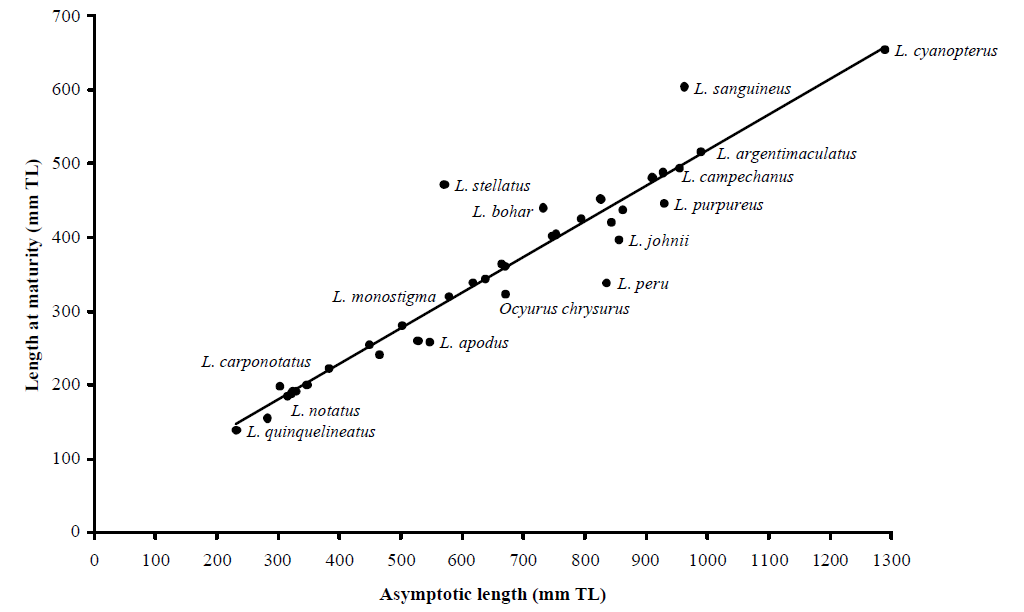
\includegraphics[width=1.1\linewidth]{/root/R-project/IFishAssessmentGuide/Images/LengthMaturity_vs_AsymptoticLength.png}
\end{center}
\textbf{Figure 1.} Length at maturity vs. asymptotic length in the family of Lutjanidae.

Over the decade after Martinez-Andrade published the relationship between Lmat and Linf for a wide range of snappers, small and large, shallow and deep water species, a lot more work was done on species identification and much more information has become available for deep water snappers. This enabled Newman and others (2016) to further refine the relationship for deep water snappers as \textbf{Lmat = 0.59*Linf}. As we are analyzing deep slope fisheries at depths below 50 meters in our program, we have adopted this life history invariable value and in this guide we use the general assumption that the \textbf{snappers targeted by our deep slope fisheries mature at about 59\% of their asymptotic length}. This assumption was verified species by species, using a range of information sources, and was shown to hold for those species in our fisheries, for which reliable direct information on maturation was available.

Epinephelidae (groupers) in general mature initially as females and later in life change sex to males. This explains certain characteristics of grouper populations. Males tend to be larger on the average than females and there is usually an overall sex ratio in favor of females. There is some overlap in size distributions between males and females in most groupers, suggesting that sex change can occur over a size range rather than occurs at a very narrow size class. Size at sex change may be partly influenced by sex ratio in the population and sex change from female to male may occur at smaller sizes when larger males are rare or absent from the population.

After looking at information on maturation for a range of species of deep water groupers we concur with Newman and others (2016) that \textbf{``deep water'' groupers mature as females at a size around 46\% of Linf}. We define deep water groupers here as those species of Epinephelidae which commonly occur in deep slope fisheries catches, from waters deeper than 50 meters. We define Lmat in groupers as the female maturation size which is estimated from \textbf{Lmat = 0.46*Linf}. For most groupers sex change from female to male seems to start at around 1.33*Lmat (1.33 times size at female maturation), after the cohort has reached maximum biomass and therewith maximum fecundity. It makes evolutionary sense that sex change from female to male would not start earlier.
 
Many Lethrinids (emperors) can undergo sex change from female to male. But not all individuals seem to follow this pattern and both sexes are found over a range of sizes above the size of first maturity. Some species, like spangled emperor, sometimes change sex from female to male before they reach maturity (if they are going to change sex at all) and females and males can mature at around the same length. In general there is considerable overlap in size distributions between males and females in most emperor species, and for purposes of emperor fisheries management, it is more meaningful to define a length at maturity by species only, rather than separately for the sexes. \textbf{In general emperors seem to be maturing at about 50\% of their asymptotic length}. We have used \textbf{Lmat = 0.5*Linf} on the basis of a review of a range of information sources and applied this for our estimates of size at maturity in emperors. In most if not all cases, this general assumption showed good overlap with published ranges for maturity in emperors.

From sketchy available information we extrapolated that for most other species in our target list our best possible estimate for length at maturation would be around 50\% of the asymptotic length, as found also for emperors. Starting from the meta-analysis of snappers by Martinez-Andrade (2003) right through a range of other information sources on length at maturation, a constant of about 50\% of Linf was found to be our best estimator for length at maturation in most of our target species, except for the deep water snappers and groupers. This estimator is also confirmed by a relationship of Lmat = 0.461 * Lmax reported from another meta-analysis by Binohlan and Froese (2009). One exception to this general rule may exist for larger Carangids which are also found in the catches of the deep slope fisheries. Reliable and precise information however is scarce and we did not find enough detailed information to deviate from the general 50\% rule for carangids either.

\begin{center}
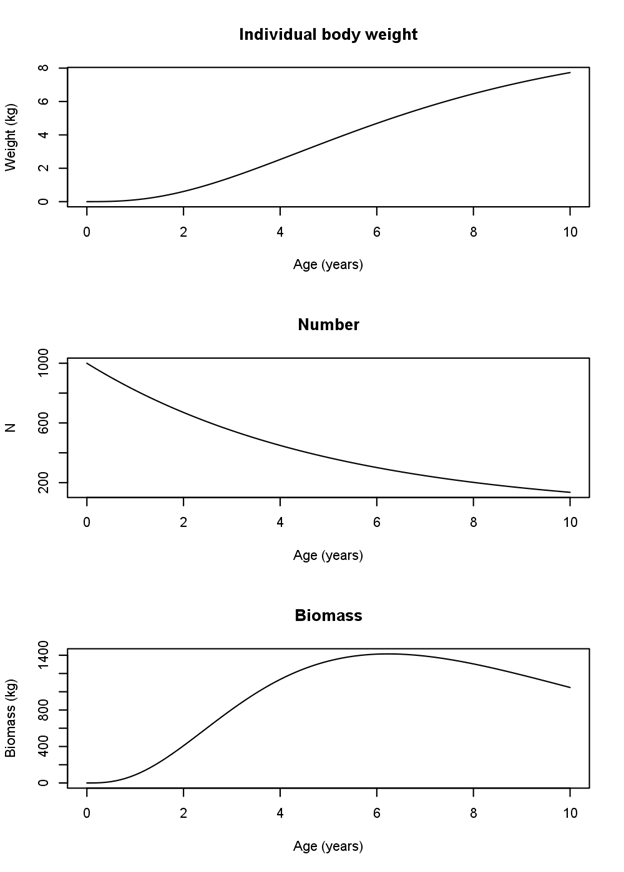
\includegraphics[width=.9\linewidth]{/root/R-project/IFishAssessmentGuide/Images/Figure-2.png}
\end{center}
\textbf{Figure 2.} The biomass of a cohort of (imaginary) fish in an un-fished situation reaches its maximum at an age (and at the related size of the fish in the cohort) where growth of individuals has slowed down to the point that it does not make up anymore for biomass loss through natural mortality.

\section{Optimum Harvest Size}
The final length-based life history characteristic that we will be using in our length-based assessment method is the \textbf{length class with the highest biomass in an un-fished population (Lopt)}. It is at this length (and corresponding age) that the biomass expressed as the number of survivors (in an un-fished cohort) multiplied with their average weight reaches a maximum (Figure 2). A fishery will obtain the maximum possible yield if it catches fish mainly around this size. Thus, fisheries managers should strive to adjust the mean length (or median length) in their catch towards this value.

Reproductive output in terms of total number of eggs (fecundity) is also optimized at this length (Lopt), where the biomass of the un-fished cohort is maximized. So also from a perspective of maximizing recruitment to the fishery, managers would strive to focus their fishery on size classes around Lopt (well beyond Lmat). And for sex-changing groupers it is important that cohorts are not decimated before sufficient individuals have changed sex from female to male, a process which begins around the size of Lopt.

Lopt can be estimated from empirical relationships between Lopt and Lmat. Lopt for catching a range of demersal fish species could be estimated as 1.33 * the length where 50\% of the fish are mature (\textbf{Lopt = 1.33 * Lmat}), based on the median values for this life history invariable (Lmat/Lopt = 0.75) over a range of demersal species (Cope and Punt, 2009). We have chosen to use this estimator of 1.33*Lmat for Lopt as the Cope and Punt (2009) study seemed to be one of the best researched situations in terms of estimating Lopt for a group of species with comparable biology and life history.
